%\documentclass[12pt]{extarticle}
\documentclass[12pt]{report}
\usepackage[utf8]{inputenc}
\usepackage{cite}
\usepackage[hyperfootnotes=false]{hyperref}
\usepackage{xcolor}
\usepackage{mathtools}
\hypersetup{
  colorlinks,
  citecolor=blue,
  linkcolor=red,
  urlcolor=blue}
\usepackage{amsmath}
\usepackage{amssymb}
\usepackage{graphicx}
\usepackage{geometry}
\usepackage{subfig}
\usepackage{bm}
%\geometry{left=30mm, right=30mm, top=30mm, bottom=30mm}
\geometry{left=35mm, right=35mm, top=35mm, bottom=35mm}
\usepackage{subfig}
\usepackage{mwe} % For dummy images
\usepackage{capt-of}
\usepackage{tabu}
\captionsetup{
	margin=1.2cm,
	format=hang,
	font=small,
	format=plain,
	labelfont={bf,up},
	textfont={it}}
\setlength{\footskip}{15mm}
\renewcommand{\thesection}{\arabic{section}}

\begin{document}
\begin{titlepage}
\newcommand{\HRule}{\rule{\linewidth}{0.5mm}} % Defines a new command for the horizontal lines, change thickness here

\center % Center everything on the page
 
%----------------------------------------------------------------------------------------
%	HEADING SECTIONS
%----------------------------------------------------------------------------------------

\textsc{\LARGE University of Liege}\\[1.5cm] % Name of your university/college
\textsc{\Large Master Thesis Summary}\\[1cm] % Major heading such as course name

%----------------------------------------------------------------------------------------
%	TITLE SECTION
%----------------------------------------------------------------------------------------

\HRule \\[0.4cm]
{ \huge \bfseries Energy-based Multi-Modal Attention}\\[0.4cm] % Title of your document
\HRule \\[1.5cm]
 
%----------------------------------------------------------------------------------------
%	AUTHOR SECTION
%----------------------------------------------------------------------------------------

\begin{minipage}{0.4\textwidth}
\begin{flushleft} \large
\emph{Author:}\\
Aurélien \textsc{Werenne } % Your name
\end{flushleft}
\end{minipage}
~
\begin{minipage}{0.4\textwidth}
\begin{flushright} \large
\emph{Supervisor:} \\
Dr. Raphaël \textsc{Marée} % Supervisor's Name
\end{flushright}
\end{minipage}\\[2cm]

% If you don't want a supervisor, uncomment the two lines below and remove the section above
%\Large \emph{Author:}\\
%John \textsc{Smith}\\[3cm] % Your name

%----------------------------------------------------------------------------------------
%	DATE SECTION
%----------------------------------------------------------------------------------------

{\large \today}\\[2cm] % Date, change the \today to a set date if you want to be precise

%----------------------------------------------------------------------------------------
%	LOGO SECTION
%----------------------------------------------------------------------------------------

\includegraphics[scale=0.2]{figs/logo}\\[1cm] % Include a department/university logo - this will require the graphicx package
 
%----------------------------------------------------------------------------------------

\vfill % Fill the rest of the page with whitespace

\end{titlepage}

\tableofcontents
\clearpage

%------------------------------------------------
\section{Introduction}
%------------------------------------------------
\indent In our daily lives we often use multiple resources to gain a maximal amount of information about a particular situation. For example, when we are at a museum admiring a painting, both the image of the painting itself as the written description next to it gives us different but complementary information. The term \textit{modality} is generally understood to mean a way in which something happens. Multimodal Deep Learning (MMDL) has received much attention in the last three years\cite{afouras, jaiswal, liu-kuan}, it aims at building models that can process and combine information from multiple modalities. One of the success stories using MMDL is the work of Afouras et al.\cite{afouras} using both audio and images of lip movements to obtain state-of-the art speech recognition results. Throughout this report we use the terms modality and mode interchangeably.\\

\indent Previous work has mostly been focused on studying the best ways to combine different modalities. A major flaw of those models is their lack of robustness in real-world settings. Indeed the quality and usefulness of the modes can vary with time, and are dependent on the context. The desired behaviour of multimodal systems would be to adapt and distribute attention to the current most relevant modes. Humans have this ability, often called \textit{cross-modal attention}\cite{crossmodal}. A situation we all have encountered in which we use cross-modal attention is the cocktail-party effect\cite{cocktail-party}, it refers to the difficulty we sometimes have understanding speech in noisy social settings. As a subconscious response, we tend to look at the mouth of our interlocutor i.e. we shift some attention from the auditory to the visual senses.\\

\indent In this work I introduce a novel deep learning mechanism, \textit{Energy-based Multi-Modal Attention} (EMMA), that aims at mimicking human's cross-modal attention. More specifically, the task of EMMA  is to decide how much attention to devote to each mode taking several factors into account: noisiness, correlations between modes, unseen/missing values. The focus of this work is not to create a new MMDL architecture, but instead to design a module to be inserted in an already-trained MMDL model in order to increase its robustness. \\

\indent The report is organized into five parts. First, section \ref{sec:problem} formalizes the goal and setting of the problem. Next, the proposed architecture is described. Section \ref{sec:regul} discusses a new regularizer to use during the training of the EMMA module. And to finish, section \ref{sec:experim} examines the results of several experiments.


%------------------------------------------------
\section{Problem Statement}\label{sec:problem}
%------------------------------------------------

A Deep Neural Network for multi-modal data $\mathbf{x}$ is typically constructed as a many-to-one encoder-decoder. Each modality goes through a different encoder extracting relevant features, those features are then fused together in the decoder. The decoder is trained to make predictions $\hat{y}$ as close as possible to the groundtruth $y$.\\

\indent We define the i.i.d. dataset $(\mathbf{x},y) \in \mathcal{D}^{(N)}$ of size $N$, all samples $\textbf{x}$ are composed of $M$ modalities. Each encoder $i$ extracts a \textit{feature vector} $\textbf{m}_i$. Multi-modal machine learning is used to solve problems if it reduces the entropy about the output as follows
\begin{equation}
I(y\,;\textbf{m}_i) \leq I(y\,;\textbf{m}_i|\{\textbf{m}_j\}_{1:M, i \neq j })
\end{equation}
A few examples of feature vectors are Fourier transforms of audio waves, flattened activation maps of Convolutional Neural Networks and context vectors produced by Recurrent Neural Networks.\\

\indent The EMMA module is inserted in between the encoders and decoder (see Fig.\ref{fig:model-with}) to apply an attention operation to every feature vector as
\begin{equation}
\textbf{m}_i' = \beta_i \textbf{m}_i \quad \text{with} \quad \beta_i \in [0,1]
\label{eq:masking}
\end{equation}
where \textit{attention factors} $\beta_i$ are a function of all the feature vectors. Intuitively, if $\beta_i$ is close to zero, the corresponding vector $\textbf{m}_i'$ will also be close to zero and thus triggers less activations. To put it in other words, the influence of a mode on predictions is decreased for a low attention factor. Low values of $\beta_i$ are desired for modes with low information but also for noisy/missing/unseen values. The latter three types of values are regrouped under the name \textit{abnormal values}. 

\begin{figure}[!ht]
    \centering
    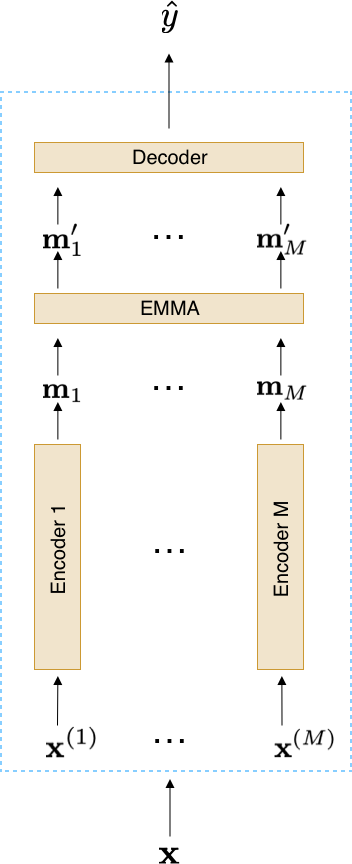
\includegraphics[scale=0.4]{figs/model-with-emma.png}%
	\vspace{1mm}\caption{A typical multi-modal model structure. The blue dashed rectangles show how an EMMA module can be inserted in between the encoders and the decoder.}%
	\label{fig:model-with}
\end{figure}

%------------------------------------------------
\section{EMMA}\label{sec:emma}
%------------------------------------------------

%------------------------------------------------
\subsection{Framework Overview}
The module is composed of three sequential steps: the \textit{Energy-}, the \textit{Composition-} and the \textit{Attention-step}. The main idea behind the three steps of the procedure are briefly outlined below. \\

\indent Energy-based models (EBM, \cite{EBM}) approximate the negative log-likelihood of the data. The approximated value is referred to as the energy, which will take low values on the data manifold and will be high everywhere else. Thus, we now have a way to quantify how normal/abnormal the modes are. However such models are difficult to optimize in practice. An alternative approach is to use De-noising Autoencoders (DAE, Vincent et al.\cite{dae-vincent}), it was shown in\cite{potentialenergy} it is possible to derive the shape of the true energy function, the so-called \textit{potential energy}. \\

\indent Potential energies help us distinguish normal from abnormal values for a specific mode, but they do not express correlations with other modes or even how important the mode is for making good predictions. A parametric function composed of potentials, \textit{modal energies}, are introduced to solve this issue. Finally, the Ising model\cite{ising-model} normalizes modal energies to the unit interval as \textit{importance weights}.\\

\indent Our attention mechanism is based on the work of the famous psychologist and economist Daniel Kahneman. He considers attention as a resource to be distributed among various stimuli\cite{kahneman}, in contrast to the more classical viewpoint where attention is a selective process. Kahneman describes attention in terms of a capacity. Accordingly, during the training EMMA will learn how much the optimal capacity is for the task, it will also find the best filtering threshold.

\begin{figure}[!hbtp]
\centering
\includegraphics[scale=0.4]{figs/three-steps.png}
\caption{High-level view of the architecture of EMMA.}
\label{fig:three-steps}
\end{figure}


%------------------------------------------------
\subsection{Energy-step}
\subsubsection*{Autoencoders and potential energy}
Autoencoders (AE) are simple models trained to attempt to copy their inputs to outputs. They are made out of two parts: an encoder $\textbf{z}_i = f(\textbf{m}_i)$ and a decoder $g(\textbf{z}_i)$. The input-to-output mapping is called the reconstruction and is written as $r(\textbf{m}_i) = g(f(\textbf{m}_i))$. In this work we use an AE of the following specific architecture:
\begin{equation}
f(\textbf{m}_i) = \sigma(W\textbf{m}_i + \textbf{b}_h)\,,
\label{eq:ae-arch1}
\end{equation}
\begin{equation}
g(\textbf{z}_i) = W^T\textbf{z}_i + \textbf{b}_r
\label{eq:ae-arch2}
\end{equation}
Using tied weights is an important constraint necessary to derive the energy function. \\

\indent In this work we use a regularized variation of the AE: the de-noising autoencoder (Vincent et al.\cite{dae-vincent}). This variation is obtained by adding a corruption process to the inputs, $\tilde{\textbf{m}}_i = \textbf{m}_i + \epsilon$ (see Fig.\ref{fig:denoising-ae}). De-noising autoencoders are then trained to minimize the reconstruction loss,
\begin{equation}
\mathcal{L}_{\text{DAE}} = \lVert r(\tilde{\textbf{m}}_i) - \textbf{m}_i \rVert_2^2
\end{equation}
Interestingly, Alain \& Bengio\cite{alainbengio} demonstrated that the reconstruction vector of a de-noising autoencoder is proportional to the score (log-likelihood),
\begin{equation}
r(\tilde{\textbf{m}}_i) - \textbf{m}_i \propto \frac{\partial \log p(\textbf{m}_i)}{\partial \textbf{m}_i}
\label{eq:score}
\end{equation}
To put it in another way, the reconstruction minus the input vector points towards the most likely corresponding de-noised input. We can visualize the vector field of reconstructions evaluated in the region around a toy data manifold  in Fig.\ref{fig:vfield}. Notably, the data manifold acts as a sink in the vector field of the input space. \\
\begin{figure}[!htbp]
  \centering
  \subfloat[Architecture]{\includegraphics[width=0.45\textwidth]{figs/denoising-ae.png}\label{fig:f1}}
  \hfill
  \subfloat[Denoising process. (Image from \cite{dae-vincent})]{\includegraphics[width=0.45\textwidth]{figs/vfield.png}\label{fig:f2}}
  \caption{Denoising Autoencoder (DAE).}
  \label{fig:denoising-ae}
\end{figure}

\indent Furthermore, Kamyshankska \& Memisevic\cite{potentialenergy} observed that those vector fields are also gradient fields, due to the fact that the integrability criterion is satisfied when using tied weights\footnote{See appendix A}:
\begin{equation}
\frac{\partial(r_k(\tilde{\textbf{m}}_i)- m_{i;k})}{\partial m_{i;l}} = \frac{\partial(r_l(\tilde{\textbf{m}}_i)- m_{i;l})}{\partial m_{i;k}}
\end{equation} 
Therefore, the vector field can be written as the derivative of a scalar field. In analogy to physics, the scalar field may then be thought of as a potential energy and the vector field as a corresponding force. \cite{potentialenergy} derives the potential energy function as,
\begin{equation}
\begin{split}
\mathrm{V}_i &= -\int (r(\tilde{\textbf{m}}_i) - \textbf{m}_i)d\textbf{m}_i  \\
&= -\int f(\textbf{m}_i)d\textbf{m}_i - \frac{1}{2} \lVert \textbf{m}_i + \textbf{b}_r \rVert_2^2 + \text{const} \\
&= -\sum_k \log(1 + \text{exp}(W_{.k}^T \textbf{m}_i + b_k^h)) + \frac{1}{2} \lVert \textbf{m}_i - \textbf{b}_r \rVert_2^2 + \text{const}
\end{split}
\end{equation}
Details of the computation can be found in Appendix B.  By simply integrating Eq.\ref{eq:score}, we can corroborate the significance of the potential energy $\mathrm{V}_i$:
\begin{equation}
\begin{split}
r(\tilde{\textbf{m}}_i) - \textbf{m}_i &\propto \frac{\partial \log p(\textbf{m}_i)}{\partial \textbf{m}_i} \\
-\int (r(\tilde{\textbf{m}}_i) - \textbf{m}_i)d\textbf{m}_i &\propto -\log p(\textbf{m}_i) \\
\mathrm{V}_i &\propto -\log p(\textbf{m}_i) + \text{constant}
\end{split}
\label{eq:shape-potential}
\end{equation}
The potential energy $\mathrm{V}_i$ is proportional to the true energy, the negative log-likelihood (if we consider the constant as the partition function).

\begin{figure}[!htbp]
\centering
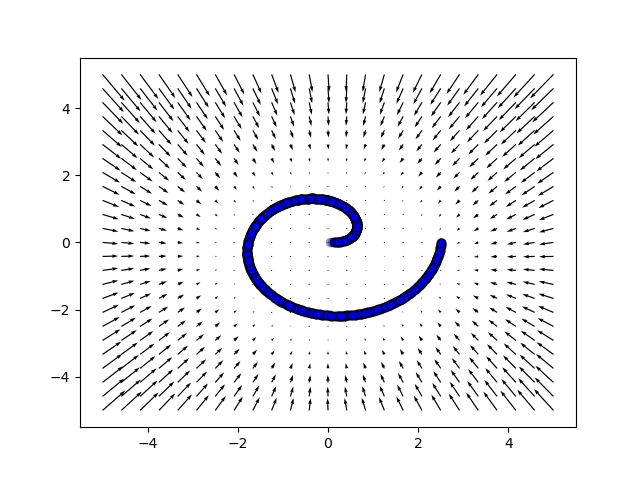
\includegraphics[scale=0.95]{figs/vector-field.png}
\caption{Vector field of the reconstruction error $r(\tilde{\textbf{m}}_i) - \textbf{m}_i$, and the samples of the data manifold. (Image from \cite{alainbengio})}
\label{fig:vfield}
\end{figure}

\subsubsection*{Abnormal values}
\indent Another interesting quantity is the Laplacian of the energy function, $\Delta \mathrm{V}_i$. It can be computed using the expression\footnote{Appendix C} below,
\begin{equation}
\Delta \mathrm{V}_i = \text{Tr}[W^T\,\text{diag}(\sigma'(W\textbf{m}_i + \textbf{b}_h))\,W] - M \quad \text{with} \quad \sigma'(x) = \sigma(x)(1-\sigma(x))
\end{equation}
The Laplacian is the divergence of the gradient and will be negative at a sink. Since we know that the data manifold behaves as a sink in its vector field, this helps us construct a simple normal/abnormal classifier,
\begin{equation}
\eta(\textbf{m}_i) = \begin{cases}
      \eta_+ & \text{if}\ \Delta \mathrm{V}_i < 0 \\
      \eta_- & \text{otherwise}
    \end{cases}
\end{equation}
We will appreciate how relevant the classifier $\eta$ is in Section \ref{sec:regul}.


%------------------------------------------------
\subsection{Composition-step}
From the previously computed potential energies we can construct composed energy functions, modal energies, of the general form
\begin{equation}
E_i = f(\mathrm{V}_i) + \sum_{k \neq i}^M g(f(\mathrm{V}_i), f(\mathrm{V}_k))
\end{equation}
The reason of this transformation is three-fold. First, the potential energies are approximations of the shape of the true negative-log likelihood (Eq.\ref{eq:shape-potential}, as a consequence potential energies are possibly be on very different scales with different biases. Secondly, as stated in \cite{alainbengio} there can be ``bad" attractors in the vector fields, leading to erroneous values of the energy function $\mathrm{V}_i$. By leveraging the correlations between the energy functions (via $g$), the modal energies can be more robust to those errors. Lastly, the parameters of the modal energies can be trained to minimize the loss with respect to predictions. For example, the function $g$ can be designed as a switch, if $g(\mathrm{V}_i, \mathrm{V}_j)$ and $g(\mathrm{V}_j, \mathrm{V}_i)$ are asymmetric.\\

\indent As a side-note, the composition step is the most ``engineered" part of the model. There are thus many other ways to design the system that could possibly obtain better results. \\

\indent A problem we overlooked so far is that we neglected the integration constant (corresponding to the partition function) in the potential energy computation. As a consequence, $\mathrm{V}_i$ is biased. To correct the bias, an easy fix is to subtract the lowest value potential energy $\mathrm{V}_{min}^{(i)}$ of the training samples. At the same time we can multiply it by a weight to solve the scaling problem:
\begin{equation}
\phi_i = w_iV_i' + b_i \,\,(= f(\mathrm{V}_i)) \quad \text{with} \quad V_i' = \max(\mathrm{e}, \mathrm{V}_i - \mathrm{V}_{min}^{(i)} + \mathrm{e})
\end{equation} 
Instead of mapping the lowest values to zero, we map it to $\mathrm{e}$, Euler's number. This is because the computation of the gradient during the optimization involves a logarithm of $\phi_i$\footnote{See appendix D}. Hence, to prevent exploding gradients we add $\mathrm{e}$. The reason we use a max-operator is because lower energy values than $\mathrm{V}_{min}^{(i)}$ can occur during inference.\\[0.38cm]

\indent Now, let us introduce the building blocks of each modal energy $i$, called \textit{partial energies}:
\begin{equation}
E_{ij} = \phi_i^{\gamma_{ij}} \phi_j^{1-\gamma_{ij}} \,\,(= g(f(\mathrm{V}_i), f(\mathrm{V}_j)))
\end{equation}
with $w_i \in \mathbb{R}^+$, $\gamma_{ij} \in [0,1]$. Note that $E_{ii} = \phi_i$. Partial energies satisfy the switch property previously discussed if we add the constraint $\gamma_{ij} = \gamma_{ji}$. As a consequence, the two modes $i$ and $j$ will be strongly dependent when $gamma_{ij}$ equals zero. At the opposite spectrum, they will be completely decoupled when gamma tends to one.\\

\indent Furthermore, modal energies are defined as sum over their respective partial energies:
\begin{equation}
E_i = \sum_{k=1}^M E_{ik}
\end{equation}
Finally, the system energy $\mathcal{S}$ is the sum of all modal energies, which can be used as an indicator of how uncertain the model is about the data.\\

\indent The importance weights are computed as likelihoods in a Gibbs distribution:
\begin{equation}
\alpha_i = \frac{1}{Z}e^{-\tau E_i} \quad \text{with the partition function} \quad Z = \sum_i^M e^{-\tau E_i} 
\label{eq:ising-model}
\end{equation}
where the \textit{coldness} $\tau$ is a hyperparameter controlling the amount of entropy in the system. At high temperature/low coldness the distribution is uniform, and at low temperature/high coldness the importance weight corresponding to the lowest energy tends to 1, while the other importance weights approach zero.

%------------------------------------------------
\subsection{Attention-step}
\subsubsection*{Attention factors}
The attention factors $\beta_i$ are determined from the importance weights:  
\begin{equation}
\beta_i = \text{ReLU}(\text{tanh}(G\alpha_i - b))
\end{equation}
where the gain ($G$) and bias ($b$) are learnable in $\mathbb{R}^+$. As previously mentioned, the output feature vectors $\mathbf{m}'_i$ are obtained by multiplying the inputs $\mathbf{m}_i$ with the factors $\beta_i$ (Eq.\ref{eq:masking}). Thus,
\begin{equation}
\text{if}\,\, \alpha_i \leq \text{threshold then}\,\, \textbf{m}'_i \approx 0 \, , \,\, \text{else}\,\, \textbf{m}'_i \rightarrow \textbf{m}_i
\end{equation}
We can distinguish those phases if we plot the activation function (see Fig.\ref{fig:tanh}). The convergence rate of $\textbf{m}'_i$ to $\textbf{m}_i$ is characterized by the gain. Whereas, the output $\textbf{m}'_i$ depends on both parameters $G$ and $b$. In particular, $\textbf{m}'_i$ is completely masked out if
\begin{equation}
\begin{split}
&\Leftrightarrow G\alpha_i - b \leq 0 \\
&\Leftrightarrow\log(\alpha_i) \leq \log(b/G)\\
&\Leftrightarrow E_i \geq \frac{\log(G/b) - \log(Z)}{\tau} 
\end{split}
\end{equation}
From the inequality we deduce coldness also influences the masking threshold. When coldness equals zero, the inequality is never verified and thus their is no masking.

\begin{figure}[!hbtp]
\centering
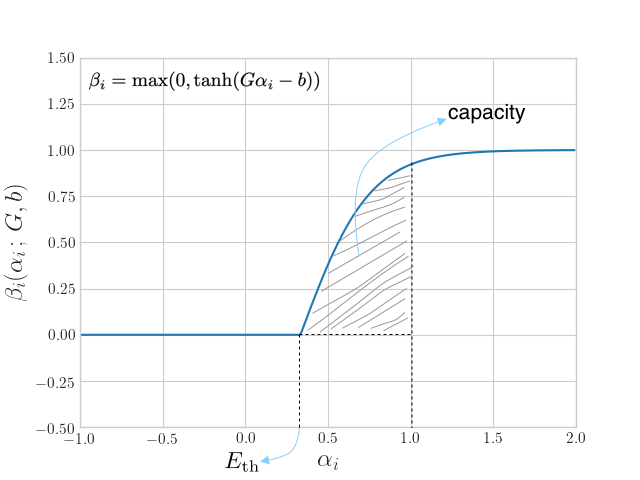
\includegraphics[scale=0.5]{figs/tanh-annotated.png}
\caption{Activation function representing the masking factor.}
\label{fig:tanh}
\end{figure}

\subsubsection*{Interpretability \& Symmetry}
The choice of having a common gain and bias is unconventional and makes the system less expressive. However, the cost of keeping them common is motivated by two properties:
\begin{itemize}
\item \textit{Interpretability}: one nice advantage of EMMA is its interpretability, indeed importance weights quantify how much attention is applied to each mode. Using separate gains and biases makes importance weights less meaningful.
\item \textit{Symmetry}: using separate parameters $G_i$, $b_i$ breaks the symmetry of the attention operation. To illustrate this, take the case where we have two modalities, one contributing in general much more (strong mode) than the other one (weak mode). The learned masking factors would look approximately as draw in Fig.\ref{fig:mask-weak-strong}. For most samples attention will work as desired. However a problem occurs if the sample has a noisy strong mode: even though $\alpha_{\text{weak}} \approx 1$, its corresponding factor $\beta_{\text{weak}}$ is still small. As a consequence, both modes will be masked out. 
\end{itemize}

\begin{figure}[!htbp]
  \centering
  \includegraphics[scale=0.67]{figs/tanh.png}
  \caption{Asymmetric effect.}
  \label{fig:mask-weak-strong}
\end{figure}


%------------------------------------------------
\section{Regularization}\label{sec:regul}\label{sec:regul}

To avoid modal energies to be too different from their original potential energies, I introduce a regularization term based on the classifier $\eta$. The loss per sample is written as,
\begin{equation}
\tilde{\mathcal{L}} = \mathcal{L}(y,\hat{y}) - \lambda \Omega \quad \text{with} \quad \Omega = \sum_{k=1}^M \eta(\textbf{m}_k) \log(\alpha_k)
\label{eq:general}
\end{equation}
Intuitively, normal/abnormal modes have positive/negative $\eta$, thus as an effect of $\Omega$ the importance weights $\alpha_i$ will be maximized/minimized. Additionally, we show below that under some conditions $\Omega$ operates as a contrastive divergence optimization.\\[0.38cm]

\indent Let $\theta = \{ \bm{\gamma}, \mathbf{w}, \mathbf{b}\}$ be the set of all parameters of the composition step. Now we can compute the gradient of the regularizer with respect to those parameters,
\begin{equation}
\nabla_{\theta} \Omega =\sum_{k=1}^M \eta(\textbf{m}_k) \nabla_{\theta} \log(\alpha_k) 
\label{eq:dev}
\end{equation}
The gradient of the logarithm becomes
\begin{equation}
\begin{split}  
\nabla_{\theta}  \log(\alpha_k) &= \nabla_{\theta} \log \bigg[ \frac{e^{-\tau E_k}}{Z} \bigg] \\
&=  \nabla_{\theta}(-\tau E_k) -  \nabla_{\theta} \log \sum_{l=1}^M e^{-\tau E_l} \\
&=  -\tau \nabla_{\theta}E_k - \frac{\sum_{l=1}^M \nabla_{\theta} e^{-\tau E_l}}{\sum_{l=1}^M e^{-\tau E_l}} \\
&= -\tau \nabla_{\theta}E_k + \tau \frac{\sum_{l=1}^M \nabla_{\theta}(E_l) e^{-\tau E_l}}{\sum_{l=1}^M e^{-\tau E_l}} \\
&= \tau \Bigg[ -\big(1 - \frac{e^{-\tau E_k}}{Z}\big)\nabla_{\theta}E_k + \sum_{l \neq k}^M \frac{e^{-\tau E_l}}{Z} \nabla_{\theta}E_l \Bigg] \\
&= \tau \Bigg[ -\big(1 - \alpha_k\big)\nabla_{\theta}E_k + \sum_{l \neq k}^M \alpha_l \nabla_{\theta}E_l \Bigg] \\
\end{split}
\label{eq:grad-log}
\end{equation}
We take the part of the gradient relative to the specific subset of parameters $\theta_i = \{[\gamma_{ik}]_{k=1}^M, w_i, b_i\}$. Equation \ref{eq:grad-log} can be split as follows
\begin{equation}
\nabla_{\theta_i}  \log(\alpha_k) = \begin{cases}
      -\tau(1-\alpha_i)\nabla_{\theta_i}E_i, & \text{if}\, i = k \\
       \tau\alpha_i\nabla_{\theta_i}E_i, & \text{if}\, i \neq k
    \end{cases}
\label{eq:log-split}
\end{equation}
Let us define $M' = \lfloor \frac{M+1}{2} \rfloor$, the number of normal modes in the sample during the training phase. Next, by substituting (\ref{eq:log-split}) in (\ref{eq:dev}) and extrapolating the sums we obtain the expression of $\nabla_{\theta_i}\Omega$ if mode $i$ is normal
\begin{equation}
\eta_+\big[ -\tau(1-\alpha_i)\nabla_{\theta_i}E_i \big] + \big[(M'-1)\eta_+ + (M-M')\eta_-\big]\alpha_i\tau\nabla_{\theta_i}E_i
\label{eq:normal-exp}
\end{equation}
and $\nabla_{\theta_i}\Omega$ if i is abnormal 
\begin{equation}
\eta_-\big[ -\tau(1-\alpha_i)\nabla_{\theta_i}E_i \big] + \big[M'\eta_+ + (M-M'-1)\eta_-\big]\alpha_i\tau\nabla_{\theta_i}E_i
\label{eq:abnormal-exp}
\end{equation}
Which can be summarized into the following equation if we pose $\eta=+1$ and $\eta=-1$:
\begin{equation}
\boxed{\nabla_{\theta_i}\Omega = -\big[(M-2M')\alpha_i + \text{sign}(\eta_i)\big]\tau\nabla_{\theta_i}E_i}
\end{equation}
Two cases can be distinguished:
\begin{itemize}
\item If the total number of modes $M$, is even then
\begin{equation}
\nabla_{\theta_i}\Omega = -\text{sign}(\eta_i)\tau\nabla_{\theta_i}E_i
\label{eq:even-M}
\end{equation}
Minimizing the loss function $\tilde{\mathcal{L}}$, will maximize the regularizer $\Omega$. Ignoring the second-order terms in the Taylor expansion of modal energies, we can conclude from equation (\ref{eq:even-M}) that gradient descent will update values of the energy function $E_i$ downward/upward for normal/abnormal inputs. 

\item If $M$ is uneven,
\begin{equation}
\nabla_{\theta_i}\Omega = \begin{cases}
      -(1-\alpha_i)\tau\nabla_{\theta_i}E_i & \text{if input $i$ is normal}  \\
      (1+\alpha_i)\tau\nabla_{\theta_i}E_i & \text{otherwise}
    \end{cases}
\label{eq:uneven-M}
\end{equation}
In analogy, modal energies are forced to stay close to their original potential energies. Additionally, an interesting phenomenon occurs: high energies that have to be low and low energies that have to be high will have stronger gradients than their counterparts. This corresponds to the positive and negative phase in contrastive divergence optimization.
\end{itemize}
%------------------------------------------------
\newpage
\section{Experiments \& Results}\label{sec:experim}
\subsection{Experiment 1}
In this experiment we train a DAE as described by equations \ref{eq:ae-arch1} and \ref{eq:ae-arch2} on manifolds in a two-dimensional space. The autoencoder has 8 hidden units and is trained on 4 types of manifolds:
\begin{itemize}
\item Linear manifold (first row of Fig.\ref{fig:result-exp1})
\item Sinus manifold (second row of Fig.\ref{fig:result-exp1})
\item Circular manifold (third row of Fig.\ref{fig:result-exp1})
\item Spiral manifold (fourth row of Fig.\ref{fig:result-exp1})
\end{itemize}\vspace*{0.5cm}

\indent We can observe from the results that the data distribution is more or less captured in the vector field of the autoencoder. Moreover, we can clearly see a false positive for the reconstruction of the linear manifold. This is because the erroneous region is a source in the vector field, which will thus be reflected in the reconstruction (small norm) but not in the potential heatmap. \textcolor{red}{Néanmoins on n'obtient pas des résultats aussi précis que dans la FIg.\ref{fig:vfield} par exemple. Il y a deux raisons à ce problème. Premièrement, je me suis rendu compte d'un léger bug dans le design du corruption process, ce qui cause le vecteurs à être plus dirigés vers le centre du manifold que vers les extrèmités. Et deuxièment, je n'ai pas beaucoup joué avec la capacité du modèle et tester d'autres fonctions d'activations.}

\begin{table}[!ht]
\centering
\begin{tabu}to \textwidth {X[l]X[c]X[r]}
  \includegraphics[width=50mm]{figs/exp1/vfield-1}
  &\includegraphics[width=50mm]{figs/exp1/energy-log-1}
  &\includegraphics[width=50mm]{figs/exp1/reconstruction-1}\\
  \includegraphics[width=50mm]{figs/exp1/vfield-2}
  &\includegraphics[width=50mm]{figs/exp1/energy-log-2} 
  &\includegraphics[width=50mm]{figs/exp1/reconstruction-2} \\
  \includegraphics[width=50mm]{figs/exp1/vfield-3} 
  &\includegraphics[width=50mm]{figs/exp1/energy-log-3}
  &\includegraphics[width=50mm]{figs/exp1/reconstruction-3} \\
  \includegraphics[width=50mm]{figs/exp1/vfield-4}\captionof{figure}{Vector field} 
  &\includegraphics[width=50mm]{figs/exp1/energy-log-4}\captionof{figure}{Potential (log-scale)} 
  &\includegraphics[width=50mm]{figs/exp1/reconstruction-4}\captionof{figure}{Reconstruction norm (log-scale)} \\
\end{tabu}
\caption{Results of experiment 1}
\label{fig:result-exp1}
\end{table}

\clearpage
\subsection{Experiment 2}
In this second experiment we augment the capacity of our autoencoder and we train it on the zero digits of the MNIST dataset. We then perform two tests:
\begin{itemize}
\item How does the potential energy evolve on a sample (100 zero images) with more and more noise? (Fig.\ref{fig:noise-energy})
\item How does the potential energy change on a sample of seen data (0 digit) versus a sample of unseen data (1 digit)? (Fig.\ref{fig:seen-unseen})
\end{itemize}

\begin{figure}[!htbp]
  \centering
  \includegraphics[scale=0.50]{figs/exp4/noise_vs_energy}
  \caption{Noise versus potential energy. Error bands represent two times the standard deviation.}
  \label{fig:noise-energy}
\end{figure}

\begin{figure}[!htbp]
  \centering
  \includegraphics[scale=0.50]{figs/exp4/seen_vs_unseen}
  \caption{Unseen/seen data and potential energy.}
  \label{fig:seen-unseen}
\end{figure}

%------------------------------------------------
\clearpage
\newpage
\section{Appendix}\label{sec:appendix}
Appendix A, B and C are developments made by \cite{potentialenergy} and adapted to our formalism.

\subsection*{Appendix A}
The integrability criterion holds since
\begin{equation}
\begin{split}
\frac{\partial(r_k(\tilde{\textbf{m}}_i)- m_{i;k})}{\partial m_{i;l}} &= \sum_j W_{kj} \frac{\partial\sigma(W\tilde{\mathbf{m}}_i + \mathbf{b}_h)}{\partial(W\tilde{\mathbf{m}}_i + \mathbf{b}_h)}W_{lj} - \delta_{kl} \\
&= \frac{\partial(r_l(\tilde{\textbf{m}}_i)- m_{i;l})}{\partial m_{i;k}}
\end{split}
\end{equation} 
where $\delta_{kl}$ denotes the Kronecker delta.

\subsection*{Appendix B}
\begin{equation}
\begin{split}
\mathrm{V}_i &= -\int (r(\tilde{\textbf{m}}_i) - \textbf{m}_i)d\textbf{m}_i  \\
&= -\int (W^T\sigma(W\textbf{m}_i + \textbf{b}_h)+\textbf{b}_r - \textbf{m}_i)d\textbf{m}_i \\
&= -W^T\int \sigma(W\textbf{m}_i + \textbf{b}_h)d\textbf{m}_i - \int (\textbf{b}_r - \textbf{m}_i)d\textbf{m}_i \\
\end{split}
\end{equation}
Let $\textbf{u} = W\textbf{m}_i + \textbf{b}_h$ be the auxiliary variable such that
\begin{equation}
\frac{d\textbf{u}}{d\textbf{m}_i} = W^T \Leftrightarrow d\textbf{m}_i = W^{-T}d\textbf{u}
\end{equation}
we can write,
\begin{equation}
\begin{split}
\mathrm{V}_i &=-\int W^TW^{-T}\sigma(\textbf{u})d\textbf{u} - \textbf{b}_r^T\textbf{m}_i +\frac{1}{2}\lVert \textbf{m}_i \rVert_2^2 + \text{const} \\
&= -\int \sigma(\textbf{u})d\textbf{u} + \frac{1}{2}\lVert \textbf{m}_i - \textbf{b}_r \rVert_2^2 + \text{const} \\
&= -\int (1+ e^{-\textbf{u}})^{-1}d\textbf{u} + \frac{1}{2}\lVert \textbf{m}_i - \textbf{b}_r \rVert_2^2 + \text{const} \\
&= -\sum_k\log (1+e^{W_{.k}^T\textbf{m}_i + b_k^h}) + \frac{1}{2}\lVert \textbf{m}_i - \textbf{b}_r \rVert_2^2 + \text{const} \\
\end{split}
\end{equation}

\subsection*{Appendix C}
The Laplacian of the potential energy is defined as
\begin{equation}
\mathrm{V}(\textbf{m}_i) = \sum_k \frac{\partial^2\mathrm{V}_i}{\partial m_{i;k}^2}
\end{equation}
If we know that,
\begin{equation}
\frac{\partial\mathrm{V}_i}{\partial \textbf{m}_i} = r(\textbf{m}_i) - \textbf{m}_i = W^T\sigma(W\textbf{m}_i) - \textbf{m}_i
\end{equation}
The Laplacian can be written as
\begin{equation}
\begin{split}
\frac{\partial^2\mathrm{V}_i}{\partial \textbf{m}_i^2} &= W^T\text{diag}(\sigma'(\textbf{m}_i))W - I_M \\
&= \text{Tr}\big[W^T\text{diag}(\sigma'(\textbf{m}_i))W\big] - M
\end{split}
\end{equation}

\subsection*{Appendix D}
The gradient of the loss with respect to $\gamma_{ij}$ is computed with the chain rule:
\begin{equation}
\frac{\partial \mathcal{L}}{\partial \gamma_{ij}} = \frac{\partial \mathcal{L}}{\partial E_i} \cdot \frac{\partial E_i}{\partial \gamma_{ij}} + \frac{\partial \mathcal{L}}{\partial E_j} \cdot \frac{\partial E_j}{\partial \gamma_{ij}} 
\end{equation}
Furthermore,
\begin{equation}
\begin{split}
\frac{\partial E_i}{\partial \gamma_{ij}} &= \frac{\partial}{\partial \gamma_{ij}} \sum_{k=1}^M E_{ik} \\
&= \frac{\partial E_{ij}}{\partial \gamma_{ij}} \\
&= \frac{\partial}{\partial \gamma_{ij}}(\phi_i^{\gamma_{ij}} \phi_j^{1-\gamma_{ij}})\\
&= \phi_i^{\gamma_{ij}}\frac{\partial}{\partial \gamma_{ij}}\phi_j^{1-\gamma_{ij}} + \phi_j^{1-\gamma_{ij}}\frac{\partial}{\partial \gamma_{ij}}\phi_i^{\gamma_{ij}}\\
&= \phi_i^{\gamma_{ij}}\phi_j^{1-\gamma_{ij}}(\log\phi_i + \log\phi_j)\\
\end{split}
\end{equation}
\clearpage

%------------------------------------------------
%------------------------------------------------
\bibliographystyle{plain}
\bibliography{biblio}

\end{document}
